\documentclass[11pt,a4paper]{article}
\usepackage[T1]{fontenc}
\usepackage[utf8]{inputenc}
\usepackage{lmodern,microtype,graphicx,xcolor,booktabs,caption}
\usepackage[hyphens]{url}
\usepackage[margin=2.5cm]{geometry}
\newcommand{\todo}[1]{\textcolor{red}{[TODO: #1]}}
\emergencystretch=2em
\begin{document}

\noindent\textbf{Letter to the Editor}

\medskip
\noindent\textbf{Crude and age-standardised asthma mortality in Brazil, 2014--2021: a reanalysis of public data}

\medskip
\noindent \todo{authors, affiliations, corresponding author}

\bigskip
\noindent To the Editor,

\medskip
Brum et al.\ reported 18,584 asthma deaths in Brazil between 2014 and 2021 and an increase in mortality of about 2.5\% per year \cite{antunes2024}. The authors shared their analysis code \cite{antunescode}, which allowed us to repeat the analysis with the same public data \cite{sim}. We reproduced the death count (18,583 deaths above 6 years of age, a difference of one) and the direction and significance class of the age-specific trends. We then asked two further questions that the crude rate cannot answer: whether the increase persists after direct age standardisation, and whether it is present in younger adults, in whom the burden is small but avoidable.

The crude national rate increased in our reproduction from 1.01 to 1.14 per 100,000 between 2014 and 2021 (+12.5\%; Table~1; slope 0.025 per 100,000 per year, 95\% CI 0.004 to 0.046; $p=0.029$). Deaths at 60 years or older make up 68\% of the total in both analyses, and the death rate at those ages is about ten times higher than at 18--59 years \cite{antunes2024}. A crude rate is therefore sensitive to the age structure of a population that is ageing. Using the 2014 Brazilian population by single year of age as the standard \cite{ibge2018}, the age-standardised rate for ages 7 and above changed from 1.12 to 1.08 per 100,000 ($-4.0\%$; slope 0.0002 per year, 95\% CI $-0.021$ to 0.022; $p=0.98$). Count models with a population offset gave an age-adjusted annual change between 0\% and +0.9\% depending on the model, with wide intervals. These estimates are compatible with no change in age-specific mortality and with a small increase, and they do not support the size of the national increase suggested by the crude series.

The pattern was different at 5--34 years. The rate rose from 0.182 to 0.219 per 100,000 (+20.3\%; slope 0.0080 per year, 95\% CI 0.0023 to 0.0138; $p=0.014$), from 182 deaths in 2014 to 210 in 2021 (Table~1, Figure~1). A control group restricted to ages 7--34, which matches the age filter of the original study, gave a similar result (+23.5\%; $p=0.011$). The group aged 35--59 years rose by 15.5\% but not significantly ($p=0.13$). A quasi-Poisson model estimated an annual increase of 4.0\% at 5--34 years ($p=0.013$), and using the WHO standard population \cite{ahmad2001} gave +16.9\% ($p=0.020$). Replacing the denominators with the post-Census projection did not change these conclusions.

\begin{table}[ht]
\centering\footnotesize
\resizebox{\textwidth}{!}{\begin{tabular}{lrrrrlr}
\toprule
Series & Rate 2014 & Rate 2021 & Change (\%) & Slope$^{a}$ & 95\% CI & $p$ \\
\midrule
Crude national rate & 1.012 & 1.138 & +12.5 & 0.0250 & (0.0036 to 0.0463) & 0.029 \\
Age-standardised (Brazil 2014) & 1.123 & 1.078 & $-$4.0 & 0.0002 & ($-$0.0213 to 0.0217) & 0.983 \\
Ages 5--34 & 0.182 & 0.219 & +20.3 & 0.0080 & (0.0023 to 0.0138) & 0.014 \\
Ages 7--34 & 0.181 & 0.224 & +23.5 & 0.0094 & (0.0031 to 0.0156) & 0.011 \\
Ages 35--59 & 0.719 & 0.830 & +15.5 & 0.0221 & ($-$0.0089 to 0.0532) & 0.132 \\
\bottomrule
\end{tabular}
}
\caption{Trend estimates, Brazil, 2014--2021. $^{a}$Change in the rate, per 100,000 per year, from a linear model on eight annual rates (95\% CI from the $t$ distribution, 6 degrees of freedom). Change (\%) is the relative change between 2014 and 2021.}
\end{table}

\begin{figure}[ht]
\centering
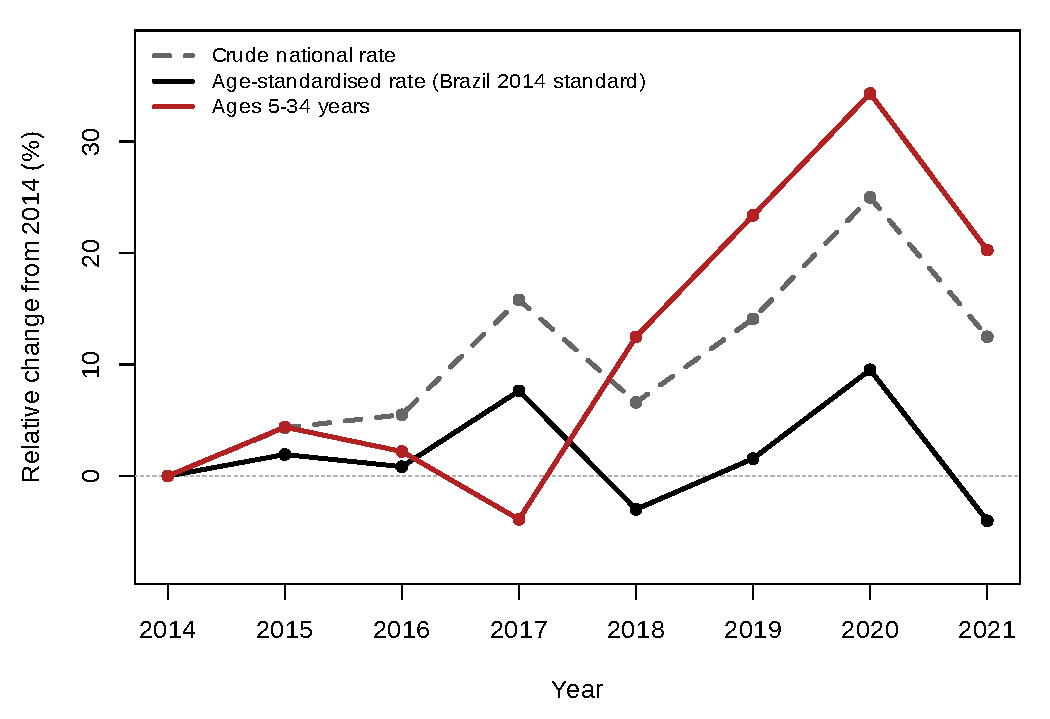
\includegraphics[width=0.8\textwidth]{figures/fig1_relative_change.pdf}
\caption{Relative change in asthma mortality from 2014, Brazil, 2014--2021. Crude national rate, age-standardised rate (Brazil 2014 standard, ages 7 and above) and rate at ages 5--34 years. Data: SIM and IBGE projections.}
\end{figure}

These results have limits. The design is ecological and descriptive, with eight annual points, and the 5--34 group is based on 182 to 210 deaths a year. The count models, the WHO standard and the alternative denominators were run after the main analyses and should be read as robustness checks. Our population denominators differ from those of the original study, so our rates are 2\% to 5\% lower and the percentage changes by age group are not identical to those published, although their signs and significance agree. We also cannot exclude changes in certification or coding practices over the period.

We read these results as complementary to the original findings. The mortality burden in Brazil remains concentrated in older adults, and the crude series suggests a rise that mostly disappears when the age structure is held fixed. At the same time, the increase in younger adults and adolescents is a signal that merits attention, because asthma deaths at those ages are rare in absolute terms and a sustained rise would be informative. Reporting age-standardised rates next to crude rates would make future surveillance comparable across years and regions. The code, intermediate tables and an audit of every decision are public at \url{https://github.com/EduIntellect/asthma-mortality-brazil-reanalysis}.

\medskip
\noindent\todo{funding, conflict of interest, author contributions as required by the journal. Ethics: only public, de-identified data were used.}

\begin{thebibliography}{9}
\bibitem{antunes2024} Brum M, Henz J, Boeira M, Soares S, Friedrich F, Pitrez PM. Recent increase in asthma mortality in Brazil: a warning sign for the public health system. J Bras Pneumol. 2024;50(5):e20240138. doi:10.36416/1806-3756/e20240138
\bibitem{antunescode} Brum M, et al. Analysis code accompanying reference~\cite{antunes2024}. GitHub repository, commit 8d527a5. \url{https://github.com/mobrant94/asthma_mortality}
\bibitem{sim} Ministério da Saúde (Brasil). Sistema de Informação sobre Mortalidade (SIM). Portal de Dados Abertos do SUS. \url{https://dadosabertos.saude.gov.br/dataset/sim}
\bibitem{ibge2018} Instituto Brasileiro de Geografia e Estatística. Projeção da População do Brasil e das Unidades da Federação, revisão 2018. \url{https://ftp.ibge.gov.br/Projecao_da_Populacao/Projecao_da_Populacao_2018/}
\bibitem{ahmad2001} Ahmad OB, Boschi-Pinto C, Lopez AD, Murray CJL, Lozano R, Inoue M. Age standardization of rates: a new WHO standard. GPE Discussion Paper Series No. 31. Geneva: World Health Organization; 2001.
\end{thebibliography}
\end{document}
